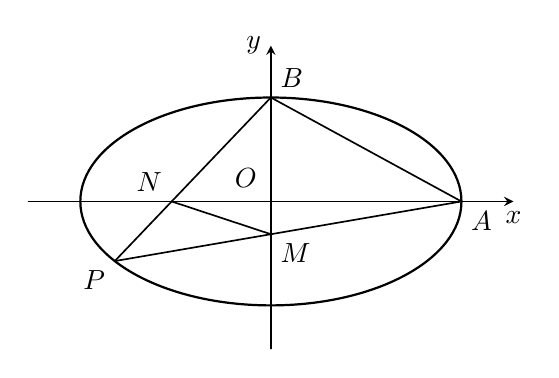
\begin{tikzpicture}[baseline,line cap=round,line join=round,>=stealth,scale=1.1]
  \def\a{2.2}
  \def\b{1.2}

  % Axes
  \draw[->,line width=0.5pt] (-2.8,0) -- (2.8,0) node[below] {$x$};
  \draw[->,line width=0.5pt] (0,-1.7) -- (0,1.8) node[left] {$y$};
  \node[above left] at (-0.05,0.05) {$O$};

  % Ellipse
  \draw[line width=0.8pt] (0,0) ellipse (\a cm and \b cm);

  % Coordinates
  \coordinate (A) at (\a,0);
  \coordinate (B) at (0,\b);

  % P in third quadrant
  \def\angP{215}
  \coordinate (P) at ({\a*cos(\angP)},{\b*sin(\angP)});

  % Intersections: M on y-axis, N on x-axis
  \coordinate (M) at (intersection of P--A and 0,-2--0,2);
  \coordinate (N) at (intersection of P--B and -3,0--3,0);

  % Segments forming the quadrangle ABNM and lines
  \draw[line width=0.6pt] (P) -- (A);
  \draw[line width=0.6pt] (P) -- (B);
  \draw[line width=0.6pt] (A) -- (B);
  \draw[line width=0.6pt] (M) -- (N);

  % Labels
  \node[below right] at (A) {$A$};
  \node[above right] at (B) {$B$};
  \node[below left] at (P) {$P$};
  \node[below right] at (M) {$M$};
  \node[above left] at (N) {$N$};
\end{tikzpicture}
